% Properties
\subsection{Leverage by Design}
%Inherent to the system...
The banking industry in this country and in most others world-wide is inherently leveraged.  Fractional-reserve banking has become a standard practice, in which a commercial depository bank can lend out a multiple of the funds it claims as assets.  Fractional-reserve banking allows for the expansion of credit during prosperous times.  Banks lend a regulated multiple of their assets out as new loans, and as the asset base value appreciates the bank may loan out an additional multiple of this appreciation.  The opposite is true in difficult economic times, where a bank may have over-valued its assets or have seen a depreciation in the value of the assets on which a lending ratio is set.  In an economic downturn the bank's asset devaluation causes a spike in their fractional lending ratio; this ratio is typically set by the central banking system.  Seeing a spike in the liabilities to asset ratio, during an economic downturn, causes a phenomena known as a 'bank run.'  In a bank run, the depositors become worried that the bank will not be able to pay back their individual liability, and in a rush of anxiety all the depositors run to the bank to redeem their certificate of deposit and clear their individual liability from the bank's balance.  Bank runs are a purely behavioral response to the fear of losing saved wealth.  With the fractional-reserve banking system in place, the bank can never actually meet the simultaneous call on all depositor certificates.  

During the Great Depression bank runs caused the liquidation and corresponding devaluation of many assets.  In the process, the wealth of ordinary depositors was at risk and the entire banking system experienced record asset devaluations.  The government response was to establish the Federal Depositor Insurance Corporation (FDIC) to insure all the depositors of a depository bank.  The creation of the FDIC was a major intervention in the lassiez-faire type of capitalism that America had established and coveted for such an extended period.  The FDIC was established to protect the wealth of the ordinary citizen, but also to cultivate the best debt service systems in the world.  The use of debt service and the availability of credit is extremely useful in a growing economy.  Debt funds the expansion of public works and private ventures.  Once the FDIC was created, depository banks were protected from the illiquid nature of their longer-term loans.  One of the greatest dangers in asset valuation is the hidden risk of holding an illiquid asset.  In an economic downturn, the preference for liquidity threatens the value of illiquid assets, and may very well lead to excessive discounting of that illiquid asset.

Investment has changed drastically over the past century, and looks to continue on its current trajectory.  In lieu of depositing wealth with a depository bank, ordinary citizen have directly and indirectly begun allocating this wealth elsewhere with the promise of higher returns.  Citizens looking to grow their wealth began allocating funds in investment vehicles, that promised and delivered superior returns to that of the depository bank.  Individual citizens need not actively seek out investment vehicles, because they are already connected to them through their pension and retirement 401k funds.  The flow of wealth into these new investment vehicles is the source of many troubles for the federal government.  The former government action, establishing the FDIC, was meant to protect the wealth of the nation while at the same time giving depository banks continued protection over their illiquid loans.  Although the government sought and continues to seek preservation of the nation's wealth and general economy, it cannot protect the illiquid and extremely leveraged investment system.

%\subsubsection{Investment Strategies}
\subsubsection{Long Wave: Market Level of Investment}  
Hedge funds, mutual funds, unit investment trusts, and money market funds are all relatively new in the field of economics.  The coordinated rise of these new time-sensitive investment vehicles and their mass adoption by the people of the United States is revolutionary in economics.  The populous of this nation and the world have been illustrating the preference for investment vehicles for a very long time now.  Average citizens are taking on greater risk and illiquidity. 

\begin{figure}[H]
\centering
\begin{subfigure}{.5\textwidth}
  \centering
  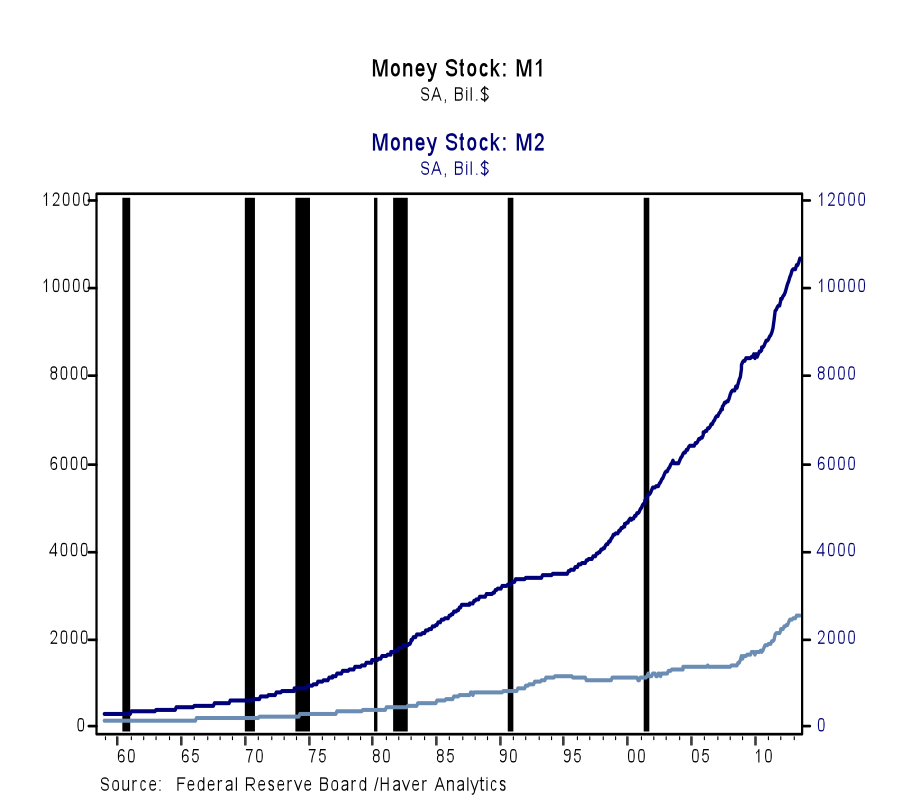
\includegraphics[width=0.9\linewidth]{figure/MoneyStockDiv.png}
  \caption{Uni-scale M1 and M2}
  \label{fig:FM}
\end{subfigure}%
\begin{subfigure}{.5\textwidth}
  \centering
  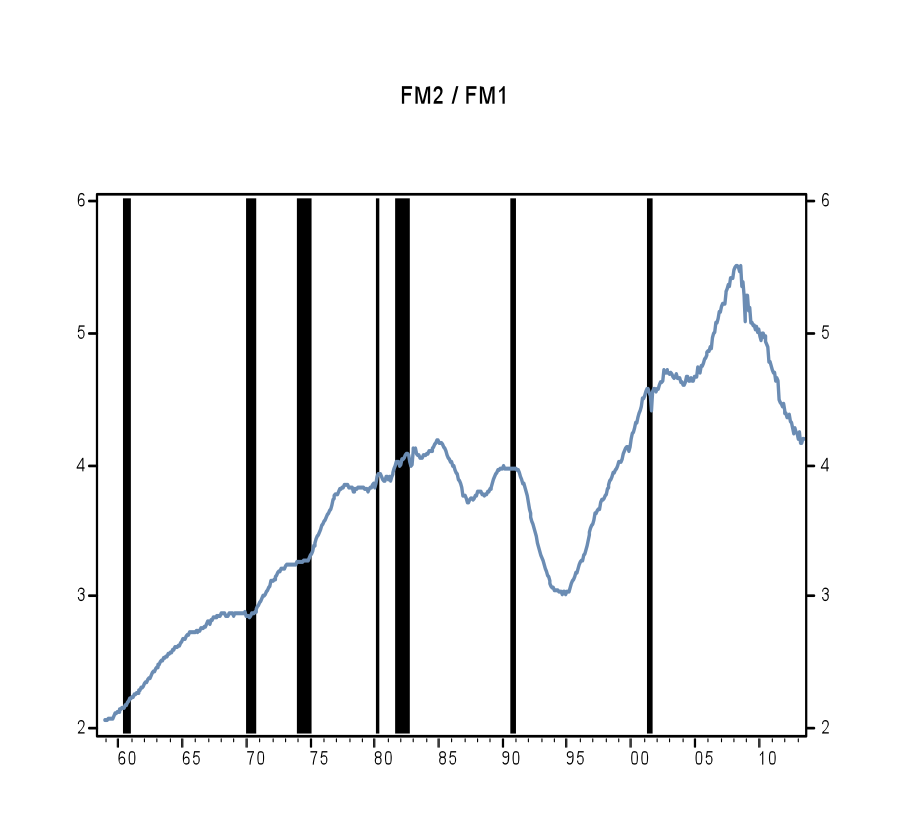
\includegraphics[width=0.9\linewidth]{figure/HistoricalFM.png}
  \caption{M2 Divided by M1: Historic Leverage}
  \label{fig:multiple}
\end{subfigure}
\caption{Divergence of M1 and M2 Money Supply Indicators}
\label{fig:div}
\end{figure}


In figure \ref{fig:div} the M1 indicator is representative of cash and checking deposits (CDs) in the United States, taking into account the commercial banking power to create money through the practice of fractional reserve banking.  The M2 indicator is representative of all that is M1, but with the addition of ``near money,'' such as money market funds and other illiquid time-sensitive assets.  The divergence of the two indicators, occurring in the period from 1970 through 1985 and in the period from 1995 through 2007, illustrates the massive movement of citizen wealth from commercial banking CDs to more complex illiquid investment products.  The Graham-Leach-Bliley Act of 1995, repealed a portion of the Glass-Steagall Act of 1933, which prohibited any one institution from acting as any combination of an investment bank, a commercial bank, and an insurance company.  This small repeal paved the way for an entire repeal of Glass-Steagall and the corresponding divergence of M2 from M1 as illustrated by the slope in figure \ref{fig:div}.

The growing divide between traditional CDs and other illiquid assets, should be of great concern for the federal government.  Unlike the FDIC protection of illiquid CDs, these newer assets are unprotected against liquidation devaluation in economic downturns.  The newer investment assets are taking a greater share of the nations wealth year after year.  With this wealth unprotected against liquidation and the corresponding devaluation, this economy is poised for a massive devaluation of wealth not seen since the Great Depression.  


\subsection{Liquidation}
The process by which a bank is forced to regain liquidity is called a fire sale.  A fire sale is destructive for a bank because there is an enormous cost of obtaining the necessary liquidity.  Once the fire sale begins the market will catch on to the distressed bank's liquidity preference.  Bidders for the illiquid assets will low ball the distressed bank in search of extremely discounted assets and once the market is functioning efficiently, with all parties having knowledge of the fire sale, the low ball prices may be accepted by the distressed bank; it all depends on how much the distressed bank really needs the liquidity.

All of this fire selling is bad for the economy.  When bidders get away with low ball offers, the market price and value for all assets similar to the fire selling asset may become unsettled.  The lack of demand for a particular illiquid asset, may in turn lead to a devaluation across that asset class.  A simultaneous flight to liquidity by multiple market participants may trigger a viscous downward spiral in the price of many of illiquid asset types being held by financial firms.  In the unprotected world of investment vehicles, the downward spiral can be exacerbated by waves of investors cashing out of their investment positions in a frenzy to exit with the highest asset value.

The fire sale of an entire asset class, by an insolvent (bankrupted) financial firm, will increase the likelihood of a market disturbance in that asset class.  A bank is economically insolvent when the market value of its assets falls short of the value of its deposits and other debt, including derivatives liabilities. The bankrupted firm's capital (net worth) turns negative and it cannot pay off all of its creditors in full and on time.  A downward spiral is all the more a reality with a bankrupted financial firm.  Banking has historically warranted a different insolvency resolution process than applies to most other firms under the Federal Bankruptcy Code.\cite{Bliss}  Administrative processes have been devised that grant regulators authority to initiate resolution of a troubled and large financial institution, in order to protect the stability of market asset value.  